% \documentclass[a4paper, 12pt]{article}
% \usepackage[osf]{libertinus}
% \usepackage[fontsize=13pt]{scrextend} 
% \usepackage[a4paper,top=3cm,bottom=3cm,left=3cm,right=3cm]{geometry}
% \usepackage{graphicx, wrapfig} 
% \usepackage{amsmath}
% \usepackage{blindtext}
% \usepackage{fancyhdr}
% \usepackage{systeme}

% \pagestyle{fancy}
% \fancyhf{} % clear all header and footer fields
% \fancyhead[R]{Mozhegova Ekaterina, DSA-02} % Right header
% \fancyfoot[C]{\thepage} % Center footer

% \title{Homework 1}
% \author{Mozhegova Ekaterina, e.mozhegova@innopolis.university}

% \AddToHook{cmd/section/before}{\clearpage}

% \begin{document}
% \maketitle

% \textbf{Tools I used:}

% [List the tools you used here, e.g., GeoGebra, Python (Matplotlib), etc.]

% \textbf{Link to the simulation:} 

% [Provide the full URL here]

% \section{Task 1}
% \textbf{Task 1}

% \underline{Task description}

% You should find:

% You should find for \( t = [0..10] \):
% \begin{enumerate}
%     \item Simulate the move of \(\vec{O}\).
%     \item Find and draw plots \( v \), \( a \), \( a_n \), \( a_{\tau} \), \( \kappa \) (Osculating circle) with respect to \( t \); 
%     \begin{align*}
%         \vec{O} &= \begin{bmatrix} x \\ y \end{bmatrix} = \begin{bmatrix} 3 \cos(2t) \cos(t) + 0.82 \\ 3 \cos(2t) \sin(t) + 0.82 \end{bmatrix}
%     \end{align*}
%     \item Find \( y(x) \), \( \vec{v} \), \( \vec{a} \), \( \vec{a}_n \), \( \vec{a}_{\tau} \) and show it on the simulation.
% \end{enumerate}



% % 1. Simulate the move of O for t = [0..10];
% % 2. Find and draw plots v, a, a_n, a_t, k (Osculating circle) with respect to t;

% % Uncomment and complete this section if needed
% % x = 3 \cos(2t) \cos(t) + 0.82
% % y = 3 \cos(2t) \sin(t) + 0.82

% % 3. Find y(x), \vec v, \vec a, \vec a_n , \vec a_τ and show it on the simulation.

% \end{document}
% \documentclass[a4paper, 12pt]{article}
% \usepackage[osf]{libertinus}
% \usepackage[fontsize=13pt]{scrextend} 
% \usepackage[a4paper,top=3cm,bottom=3cm,left=3cm,right=3cm]{geometry}
% \usepackage{graphicx, wrapfig} 
% \usepackage{amsmath}
% \usepackage{blindtext}
% \usepackage{fancyhdr}
% \usepackage{systeme}

% \pagestyle{fancy}
% \fancyhf{} % clear all header and footer fields
% \fancyhead[R]{Mozhegova Ekaterina, DSA-02} % Right header
% \fancyfoot[C]{\thepage} % Center footer

% \title{Homework 1}
% \author{Mozhegova Ekaterina, e.mozhegova@innopolis.university}

% \AddToHook{cmd/section/before}{\clearpage}

% \begin{document}
% \maketitle

% \textbf{Tools I used:}

% [List the tools you used here, e.g., GeoGebra, Python (Matplotlib), etc.]

% \textbf{Link to the simulation:} 

% [Provide the full URL here]

% \section{Task 1}
% \textbf{Task 1}

% \underline{Task description}

% You should find:

% You should find for \( t = [0..10] \):
% \begin{enumerate}
%     \item Simulate the move of \(\vec{O}\).
%     \item Find and draw plots \( v \), \( a \), \( a_n \), \( a_{\tau} \), \( \kappa \) (Osculating circle) with respect to \( t \); 
%     \begin{align*}
%         \vec{O} &= \begin{bmatrix} x \\ y \end{bmatrix} = \begin{bmatrix} 3 \cos(2t) \cos(t) + 0.82 \\ 3 \cos(2t) \sin(t) + 0.82 \end{bmatrix}
%     \end{align*}
%     \item Find \( y(x) \), \( \vec{v} \), \( \vec{a} \), \( \vec{a}_n \), \( \vec{a}_{\tau} \) and show it on the simulation.
% \end{enumerate}



% % 1. Simulate the move of O for t = [0..10];
% % 2. Find and draw plots v, a, a_n, a_t, k (Osculating circle) with respect to t;

% % Uncomment and complete this section if needed
% % x = 3 \cos(2t) \cos(t) + 0.82
% % y = 3 \cos(2t) \sin(t) + 0.82

% % 3. Find y(x), \vec v, \vec a, \vec a_n , \vec a_τ and show it on the simulation.

% \end{document}



\documentclass{article}
\usepackage{amsmath}
\usepackage{float}
\usepackage{graphicx, wrapfig} 

% \usepackage{graphicx}

\title{Theoretical mechanics. Homework 1}
\author{Ekaterina Mozhegova}
\date{\today}

\begin{document}
\maketitle
\section{Tools}

GeoGebra, Python (Matplotlib)

\section{Task 1}

\subsection{Link to the simulation}

\subsection{Task description}
You should find:
\begin{enumerate}
    \item Simulate the move of \(\vec{O}\) for \( t = [0..10] \).
    \begin{align*}
        \vec{O} &= \begin{bmatrix} x \\ y \end{bmatrix} = \begin{bmatrix} 3 \cos(2t) \cos(t) + 0.82 \\ 3 \cos(2t) \sin(t) + 0.82 \end{bmatrix}
    \end{align*}
    \item Find and draw plots \( v \), \( a \), \( a_n \), \( a_{\tau} \), \( \kappa \) (Osculating circle) with respect to \( t \); 
    \item Find \( y(x) \), \( \vec{v} \), \( \vec{a} \), \( \vec{a}_n \), \( \vec{a}_{\tau} \) and show it on the simulation.
\end{enumerate}

\subsection{Task explanation}
It can be typed or be handwritten, or mixed. The goal, to explain step by step, how did
you solve the task. You should explain your formulas too.
I’d like to highlight, that the way how do you make a simulation is also worthy for be explained.
Assume, that you are writing it for yourself, and you will read it later.

\subsection{Plots}
5. Plots. Put needed plots. Don’t forget to make an appropriate title, legend, and axes description.
\subsection{Screenshots from simulation}

Several screenshots, in some interesting positions. Example: parabola —
midway of left branch, root, somewhere in right branch.


\section{Task 2}

\subsection{Tools used for the task}
GeoGebra

\subsection{Link to the simulation}
https://www.geogebra.org/calculator/jveychw3

\subsection{Task description}

You should solve the task, till the M point travels s:

1. Simulate this mechanism (obtain all positions of
bodies 1, 2, 3)

2. Velocity for M(draw plots for magnitudes and
show vectors on simulation);

3. Accelerations (tangent, normal, overall) for
M(draw plots for magnitudes and show vectors
on simulation);

4. Draw plots of angular velocities for 2, 3 bodies.

% If R2 = 40, r2 = 30, R{3} = 15, x = x(t) = 3 + 80t^2 , sM = 0, 5.

If \( R_2 = 40, r_2 = 30, R_3 = 15, x = x(t) = 3 + 80t^2 \), and \( s_M = 0.5 \).

\begin{figure}[H]
    \centering
    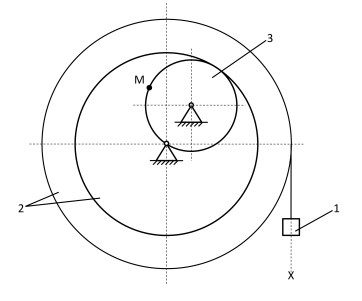
\includegraphics[width=0.5\textwidth]{Task2.png}
    \caption{Task 2\label{Task 2}}
\end{figure}

\subsection{Task explanation}

To implement a simulation, it is necessary to know the time interval. Find t by the following way:
1) \(x(t) = 3 + 80t^2 \)
\( v(x) = \dot x\)

It can be typed or be handwritten, or mixed. The goal, to explain step by step, how did
you solve the task. You should explain your formulas too.
I’d like to highlight, that the way how do you make a simulation is also worthy for be explained.
Assume, that you are writing it for yourself, and you will read it later.

\subsection{Plots}
5. Plots. Put needed plots. Don’t forget to make an appropriate title, legend, and axes description.
\subsection{Screenshots from simulation}

Several screenshots, in some interesting positions. Example: parabola —
midway of left branch, root, somewhere in right branch.


\section{Task 3}

\subsection{Link to the simulation}

\subsection{Task description}
You should find:
1. Simulate this mechanism (obtain all positions.)
(xi (t), yi (t), where i is A, B, C point)

2. Velocities for B, C (draw plots for magnitudes and
show vectors on simulation);

3. Accelerations for B and C (draw plots for
magnitudes and show vectors on simulation);

4. Draw a plot of angular velocity of body BA.

$y_A(t) = 22.5 + \sin(5\pi t)$, where $t \in [0, 10]$ sec; AB = 45, AC = 30.

\begin{figure}[H]
    \centering
    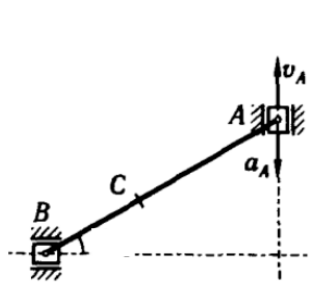
\includegraphics[width=0.5\textwidth]{Task3.png}
    \caption{Task 3}
\end{figure}


\subsection{Task explanation}
It can be typed or be handwritten, or mixed. The goal, to explain step by step, how did
you solve the task. You should explain your formulas too.
I’d like to highlight, that the way how do you make a simulation is also worthy for be explained.
Assume, that you are writing it for yourself, and you will read it later.

\subsection{Plots}
5. Plots. Put needed plots. Don’t forget to make an appropriate title, legend, and axes description.
\subsection{Screenshots from simulation}

Several screenshots, in some interesting psositions. Example: parabola —
midway of left branch, root, somewhere in right branch.


\end{document}